% ==========================================================================
\section{Computer Operation}
% ==========================================================================
    
    % ==========================================================================
    \subsection{dastaZ80DB Front Panel}
    % ==========================================================================
    \label{subsec:frontpanel}

    The dastaZ80DB has a front panel where all buttons, switches and slots are
    located for easy access. Also, in difference to the dastaZ80 Original, this
    computer has a LCD Display and some push buttons which form the
    \textit{Control Panel}.

    The front panel contains:

    \begin{itemize}
        \item ON/OFF Switch: use it to turn on and off the computer.
        \item Reset button: use it to make a reset of the computer.
        \item Micro SD Card slot: for massive storage of data.
        \item 3.5" FDD: for storage of data in floppy diskettes.
        \item Light (LED) indicators:
        \begin{itemize}
            \item Power (green): lighted when the system is switched ON.
            \item Reset (red): lighted when the system is performing a hardware
                reset.
            \item SD (purple): blinks when the SD Card is being accessed
                (read or write).
            \item Halted (yellow): lighted when the system is in Halt status.
            \item ROM Paged (blue): lighted when the ROM chip has been
                disconnected.
        \end{itemize}
        \item Control Panel
    \end{itemize}

        % ==========================================================================
        \subsubsection{Control Panel}
        % ==========================================================================
        \label{subsubsec:controlpanel}

        The Control Panel is always ON as soon as the computer has been plugged
        to the 5V/4A power supply. That's right, even when the computer is OFF,
        this panel is ON. It will make sense in a second.
        
        This Panel is used to configure some pre-booting configurations (if you
        are familiar with IBM AS/400 hardware you will see where this idea comes
        from), and also monitors the internal temperature of the box and
        switches ON and OFF a small fan used for cooling.

        The Panel consists of one LCD display and three push buttons. The
        buttons are labelled \textit{+}, \textit{-} and \textit{Select}.

        The LCD display what is called \textit{pages} of information. The
        buttons \textit{+} and \textit{-} are used to navigate the pages, and
        the button \textit{Select} is used to select a page.
        
        When plugged in, the display will show the Page 0. This is indicated by
        the number zero shown in the first character of each of the two lines of
        the display.

        Page 0 shows the Current Configuration. If the computer was to be
        switched ON at this moment, it will use the configuration displayed in
        the LCD to its boot.

        Page 0 information is:
        \[ +------------------+ \]
        \[ |0 \$0000   Clk Int| \]
        \[ |0 21.49 C   *     | \]
        \[ +------------------+ \]

        \begin{itemize}
            \item Line 1:
            \begin{itemize}
                \item \textit{0}: indicates that this is Page 0.
                \item \textit{\$0000}: refers to the address in ROM that will be
                    used to start reading the OS.
                \item \textit{Clk Int}: indicates the the Internal clock is
                    being used as system clock.
            \end{itemize}
            \item Line 2:
            \begin{itemize}
                \item \textit{0}: indicates that this is Page 0.
                \item \textit{21.49 C}: is the current measured internal
                    temperature of the box.
                \item \textit{*}: this only appears if a certain threshold of
                    maximum temperatire has been reached. If the computer is
                    switched ON, here it will appear a spinning animation
                    indicating that the fan is ON. If the computer is OFF, a
                    blinking exclamation mark will appear, indicating that it
                    may not be safe to switch on the computer.
            \end{itemize}
        \end{itemize}

        Pages 1 and 2 are selectable pages, and show the two different start ROM
        addresses that can be selected.

        \[ +------------------+ \]
        \[ |0 \$0000   Clk Int| \]
        \[ |0 21.49 C   *     | \]
        \[ +------------------+ \]
        
        To select one or the other, press the button \textit{Select} while in
        the desired page. After a couple of seconds, the Panel will display Page
        0 automatically, and you should see the selected value in its
        corresponding position.

        Pages 3 and 4 are selectable pages, and show the two different system
        clock that can be selected.

        \[ +------------------+ \]
        \[ |0 \$0000   Clk Int| \]
        \[ |0 21.49 C   *     | \]
        \[ +------------------+ \]
        
        To select one or the other, press the button \textit{Select} while in
        the desired page. After a couple of seconds, the Panel will display Page
        0 automatically, and you should see the selected value in its
        corresponding position.

        Worth noting:

        \begin{itemize}
            \item Once the computer is switched ON, the configuration cannot be
                changed. Hence, any selection via the \textit{Select} button
                will be ignored.
            \item Changes in configuration are not stored. Once the computer is
                unplugged from the power supply, it will start again with the
                default settings.
        \end{itemize}

    % ==========================================================================
    \subsection{ON/OFF button}
    % ==========================================================================
    \label{subsec:onoffbutt}

    The ON/OFF button is located on the lefthand side of the back of the
    dastaZ80 computer and on the front of the dastaZ80DB.

    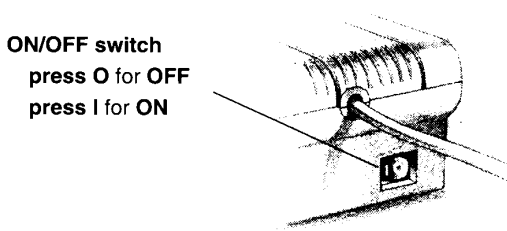
\includegraphics[scale=0.5]{images/onoffbutton.png}

    This button is used to turn ON and OFF the computer.

    Before turning it ON, read the instriuctions on the section
    \hyperref[sec:setting_system]{Setting up the system} of this manual.

    Before turning it OFF, it is highly recommended to use the command 
    \hyperref[cmd:halt]{halt} to ensure that all \textbf{DISK} data has been
    correctly saved. Otherwise, corruption of data may occur.

    % ==========================================================================
    \subsection{Reset button}
    % ==========================================================================
    \label{subsec:resetbutton}

    The reset button is located on the lefthand side of the dastaZ80 computer
    and on the front of the dastaZ80DB.

    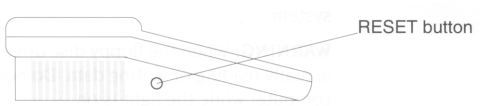
\includegraphics[scale=0.7]{images/resetbutton.png}

    This button is used to restart the computer without turning it off via the
    \hyperref[subsec:onoffbutt]{ON/OFF button}.

    To reset the computer simply press and release the button. The reset process
    will take 6.5 seconds in total, as explained in the section
    \textit{Reset circuit} of the dastaZ80 Technical Reference
    Manual\cite{dastaz80techman}.

    % ==========================================================================
    \subsection{Indicator LEDs}
    % ==========================================================================

    Indicator LEDs for the dastaZ80DB has been discussed in previous section
    \hyperref[subsec:frontpanel]{dastaZ80DB Front Panel}.

    For the dastaZ80, at the top of the computer case there a few labelled
    LEDs\footnote{A Light-Emitting Diode (LED) is a semiconductor device that
    emits light when current flows through it.} that give information of the
    status of several internal parts of the computer.

    \begin{itemize}
        \item Above the numeric pad, on the righthand side of the keyboard,
        there are two LEDs:
        \begin{itemize}
            \item \textbf{POWER}. This LED is always on when the computer is
            switched on via the \hyperref[subsec:onoffbutt]{ON/OFF button}. It glows
            in \underline{orange} colour.
            \item \textbf{DISC}. This LED blinks whenever a \textbf{DISK} operation
            (read/write) is happening. It glows in \underline{green} colour.
        \end{itemize}
    \end{itemize}
    
    \centerline{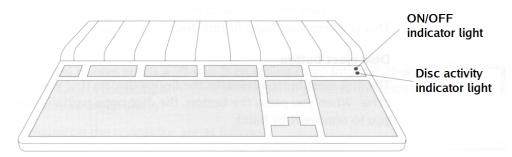
\includegraphics[scale=0.5]{images/keyboardLEDs.png}}

    \begin{itemize}
        \item Above the \textit{Esc} and function keys (\textit{F1}-\textit{F12}),
        on the lefthand side of the keyboard, there are two LEDs. These LEDs are
        multi-colour, hence glowing at different colour each:
        \begin{itemize}
            \item Computer status
            \begin{itemize}
                \item \textbf{RESET}. It glows in \underline{red} colour when
                the computer is in reset status. This happens for 6.5 seconds
                when the computer is switched ON (via the
                \hyperref[subsec:onoffbutt]{ON/OFF button}) and when the
                computer is reset via the \hyperref[subsec:resetbutton]
                {Reset button}.
                \item \textbf{HALTED}. It glows in \underline{blue} when the
                computer is in halt status. Usually after issuing the command
                \hyperref[cmd:halt]{halt}.
                \item \textbf{ROM PAGED}. It glows in \underline{green} when the
                \textbf{ROM} has been electrically disconnected and therefore
                the computer will only perform operations (read/write) from/to
                the \textbf{RAM}. This happens only during the Boot Sequence.
                See the section \textit{OS Boot Sequence} of the dastaZ80
                Programmer's Reference Guide\cite{dastaz80progref} for more
                detailed information about the Boot Sequence.
            \end{itemize}
            \item Clock Selection
            \begin{itemize}
                \item \textbf{CLOCKSEL}. It glows in \underline{yellow} colour
                when the Internal clock is used. And in \underline{purple}
                colour when an External clock is being used by the computer.
            \end{itemize}
        \end{itemize}
    \end{itemize}

    % ==========================================================================
    \subsection{MicroSD}
    % ==========================================================================

    At the back of the dastaZ80 computer and on the front of the dastaZ80DB
    there is a MicroSD slot.

    Insert here a MicroSD formatted with FAT32 and containing Disk Image
    Files formatted with DZFS\footnote{DZFS (dastaZ80 File System) is a file
    system of my own design, for mass storage devices, aimed at simplicity}.

    \centerline{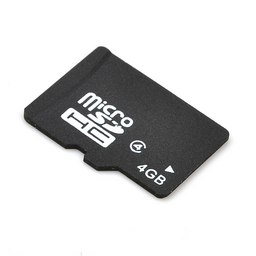
\includegraphics[scale=0.5]{images/microsdcard.png}}

    % ==========================================================================
    \subsection{3.5 inch Floppy Disc Drive}
    % ==========================================================================

    The Floppy Disc Drive is located on the righthand side of the dastaZ80
    computer and on the front of the dastaZ80DB.

    3.5 inch floppy discs can be inserted in this drive. 

    
\includegraphics[scale=0.7]{images/discslot.png}

    To remove an inserted floppy disc from the drive, press the
    \textit{Disc eject button}. The disc will partially pop out, allowing you to
    completelly remove it by hand.

    % ==========================================================================
    \subsection{Attaching peripheral devices}
    % ==========================================================================

        % ==========================================================================
        \subsubsection{TTL I/O}
        % ==========================================================================

        The dastaZ80DB has a 4 pins header labelled \textit{TTL I/O} that is
        used to connect either a TTL-to-USB cable or a TTL-to-RS-232 converter.

        This connector carries the signals for the input (keyboard) and output
        (screen).

        By connecting the dastaZ80DB to another computer, the latter can
        \textit{control} the former. As a matter of fact, there is no other way
        to input commands to the dastaZ80DB than using another device (a
        computer in most cases, but also a serial terminal can be used).

        For the output, two options are available:

        \begin{itemize}
            \item \textit{TTL}: output to a serial device (usually another
                computer running a terminal program).
            \item \textit{VGA}: output to a VGA monitor.
        \end{itemize}

        The \textit{TTL / VGA} switch (located on the \hyperref[subsec:frontpanel]
        {Front Panel}) MUST be set up to the correct position, in order to see
        output from the dastaZ80DB.

        The TTL connector pins are configured as follows (seeing it from the
        front):

        \textbf{Ground} | NC | NC | \textbf{TX} | \textbf{RX} | NC

        NC, stands for Not Connected. These are the \textit{+5V}, \textit{/CTS}
        and \textit{/RTS} signals, which are not used.



        % ==========================================================================
        \subsubsection{Dual Video Output}
        % ==========================================================================

        At the back of the computer you will find two connectors, beside each
        other, for the connection of video output.

        The first one, and necessary to use the computer, is a VGA connector for
        the \textbf{VGA video output}.
        
        Plug here a standard VGA cable connected to a VGA monitor.

        \centerline{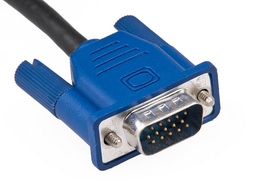
\includegraphics[scale=0.5]{images/vgaconn.png}}

        The second connector, which is optional (i.e. the computer will function
        perfectly normal without this connected), is a 3.5mm female jack for the
        \textbf{Composite video output}\footnote{The Composite video signal is
        NTSC (National Television System Committee), the standard for analog
        television used mainly in USA, Japan and some parts of South America}.

        Plug here the jack side of a 3.5mm jack-to-3-RCA Audio/Video cable
        \footnote{This is the same cable used on the Raspberry Pi for Composite
        output.}.

        \centerline{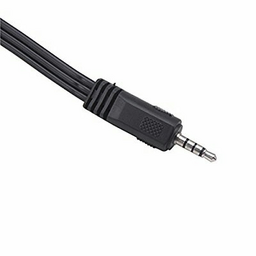
\includegraphics[scale=0.5]{images/raspicable_jack.png}}

        Connect the yellow RCA cable of the jack-to-3-RCA cable to the Composite
        input of a monitor or TV.

        \centerline{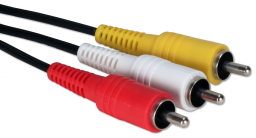
\includegraphics[scale=0.5]{images/raspicable_rca.png}}

        % ==========================================================================
        \subsubsection{Stereo Sound Output}
        % ==========================================================================

        The stereo sound signal comes out of the same connector used for the
        Composite video output.

        Connect the jack-to-3-RCA white and red cables to a pair of speakers or
        to the input of a sound system amplifier.

        % ==========================================================================
        \subsubsection{USB Keyboard for External computer}
        % ==========================================================================

        The keyboard of the dastaZ80 can be used as an USB keyboard on other
        computers.
        
        Connect the a USB cable between this connector and your other
        computer, switch on dastaZ80 and press the key \textit{ScrollLock}. From
        now on (as indicated by the ScrollLock LED being lighted) dastaZ80 will
        not read any keystrokes, but instead will send them to the computer
        connected via USB.

        If you want to use dastaZ80 at any time, just press \textit{ScrollLock}
        again. There is no need to unplug the USB cable. The \textit{ScrollLock}
        key is doing the switching.

        This feature can be handy when you are using dastaZ80 and another PC at
        the same time and don't want to be switching hands between two keyboards
        all the time. It saves space too!

        % ==========================================================================
        \subsubsection{ROM Cartridge}
        % ==========================================================================

        Refer to the section \textit{Cartridge Port} of the dastaZ80 Technical
        Reference Manual\cite{dastaz80techman} for more detailed information.

        % % ==========================================================================
        % \subsubsection{General-Purpose Input/Output (GPIO)}
        % % ==========================================================================

        % This connector exposes all CPU signals and can be used to connect external
        % devices directly to the components (e.g. \textbf{CPU}, \textbf{RAM)} of
        % the computer.